\documentclass{article}
\usepackage[utf8]{inputenc}
\usepackage[T1]{fontenc}
\usepackage[ukrainian]{babel}
\usepackage[12pt]{extsizes}
\usepackage{graphicx}
\usepackage{amsmath}
\usepackage{amsfonts}
\usepackage{multicol}
\usepackage{cmap}
\usepackage{amsthm}
\graphicspath{{pictures/}}
\DeclareGraphicsExtensions{.pdf,.png,.jpg}

\title{Регресійний аналіз}
\author{nikita.forduy }
\date{February 2020}

\usepackage{natbib}
\usepackage{graphicx}

\begin{document}
  
  \pagestyle{empty}
  \newtheorem{theorem}{Теорема}

  \begin{titlepage}
      \thispagestyle{empty}
      \setlength{\parindent}{0ex} % set paragraph indenting to zero
      
      \begin{center}
        НАВЧАЛЬНО-НАУКОВИЙ КОМПЛЕКС \\
        "ІНСТИТУТ ПРИКЛАДНОГО СИСТЕМНОГО АНАЛІЗУ" \\
        НАЦІОНАЛЬНОГО ТЕХНІЧНОГО УНІВЕРСИТЕТУ УКРАЇНИ \\
        "КИЇВСЬКИЙ ПОЛІТЕХНІЧНИЙ ІНСТИТУТ ІМЕНІ ІГОРЯ СІКОРСЬКОГО" \\
        \smallskip
        КАФЕДРА МАТЕМАТИЧНИХ МЕТОДІВ СИСТЕМНОГО АНАЛІЗУ \\
      \end{center}
      \vspace{60mm}
      
      \begin{center}
        РОЗРАХУНКОВА РОБОТА \\
        з теми "Регресійний аналіз" \\
        
      \end{center}
      
      \vspace{30mm}
      

      \hfill
      \begin{minipage}{.4\linewidth}
        \begin{flushright}
          Виконав студент групи КА-81
          Фордуй Нікіта
          \smallskip
          Перевірила Каніовська І.Ю.
        \end{flushright}
      \end{minipage}
      
      \vspace{10mm}

      \vfill
      \begin{center}
        Київ 2020
      \end{center}
      
      \setlength{\parindent}{5ex} % reset paragraph indenting
  \end{titlepage}

  \tableofcontents

  \pagestyle{plain}

  \newpage
  \section{Завдання 1}
    \subsection{Завдання}
      \begin{enumerate}
        \item Провести аналіз вибірки та вибрати підходящу лінійну регресійну модель.
        \item За методом найменших квадратів знайти оцінки параметрів вибраної моделі.
        \item На рівні значущості $\alpha$ = 0,05 перевірити адекватність побудованої моделі.
        \item Для самого малого значення параметра побудованої моделі на рівні значущості
        $\alpha$ = 0,05 перевірити гіпотезу про його значущість.
        \item Побудувати прогнозований довірчий інтервал з довірчою ймовірністю $\alpha$ = 0,95 
        для середнього значення відклику та самого значення відклику в точці x =16.
        \item Написати висновки.
      \end{enumerate}
      \begin{center}
        \begin{tabular}{| l | l | l |}
          \hline
          X & Y \\
          \hline
          1 & 18 \\
          2 & 28 \\
          3 & 7.4 \\
          4 & 32 \\
          5 & 40 \\
          6 & 60 \\
          7 & 51 \\
          8 & 33 \\
          9 & 77 \\
          10 & 34 \\
          11 & 72 \\
          12 & 48 \\
          13 & 30 \\
          14 & 77 \\
          15 & 39 \\
          16 & 52 \\
          17 & 46 \\
          \hline
        \end{tabular}
        \;\;\;\;\;\;\;\;\;\;\;\;\;\;\;\;
        \begin{tabular}{| l | l | l |}
          \hline
          X & Y \\
          \hline
          18 & 66 \\
          19 & 27 \\
          20 & 75 \\
          21 & 59 \\
          22 & 32 \\
          23 & 50 \\
          24 & 52 \\
          25 & 40 \\
          \hline
        \end{tabular}
      \end{center}
    \subsection{Аналіз вибірки та вибір регресійної моделі}
      Розглянемо розташування значень відкликів Y на площині:
      \begin{center}
        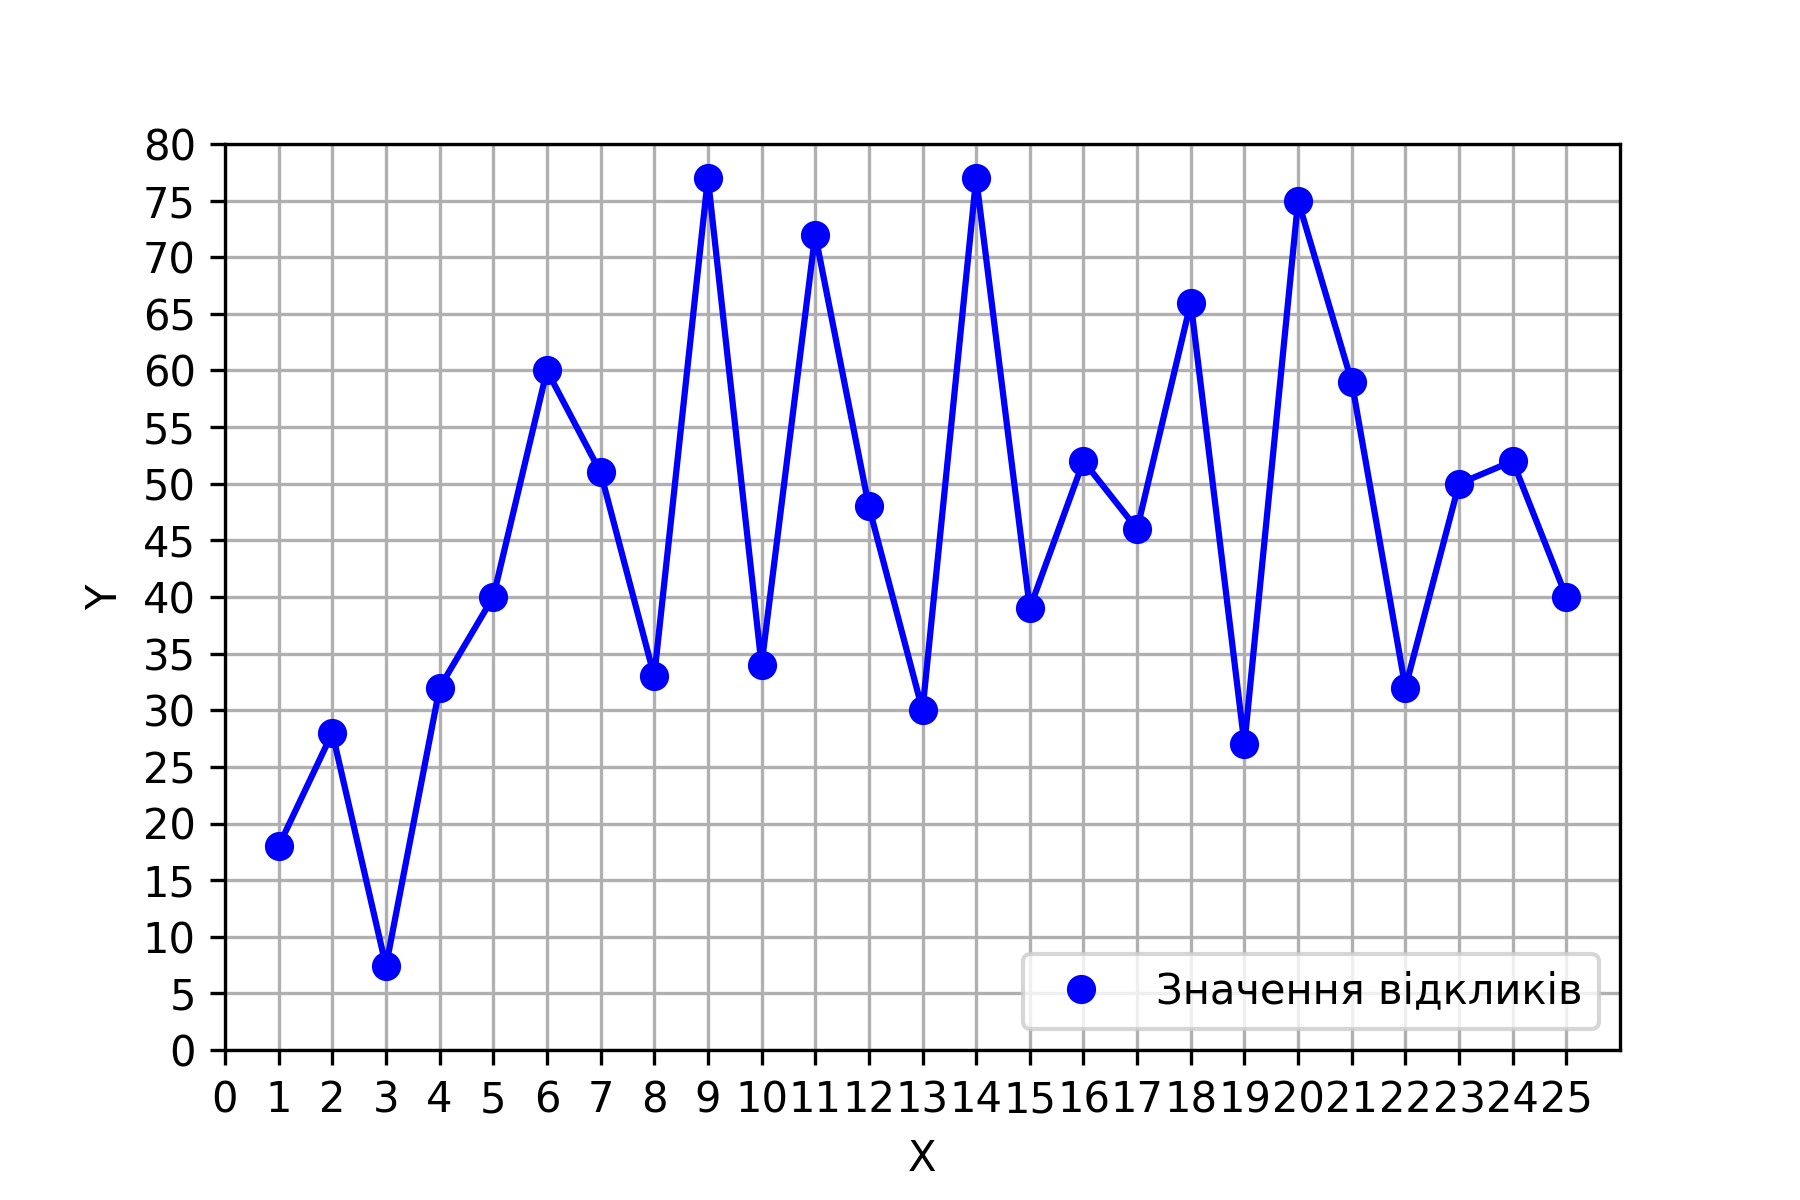
\includegraphics[scale=0.8]{task1_data}
      \end{center}
      За розташуванням значень відкликів на площині стає зрозуміло, 
      що залежність є нелінійна і схожа на квадратичну.
      Тому розглянемо модель $f(x) = \beta_0 + \beta_1 x + \beta_2 x^2$
    \subsection{Знаходження за МНК оцінки параметрів вибраної моделі}
      Матриця плану для вибраної моделі матиме вигляд:
      \begin{equation}\label{eq:}
          F = 
          \begin{pmatrix}
              1 & 1 & \dots & 1 \\
              1 & 2 & \dots & 25 \\
              1^2 & 2^2 & \dots & 25^2 \\
          \end{pmatrix}^T
      \end{equation}
      Після цього використовуємо матрицю F для знаходження іформаційної матриці 
      Фішера $A = FF^T $ та дисперсійну матрицю Фішера $A^{-1}$; обидві з них мають 
      розмір $3 \times 3$.
      Обчислені матриці наведені у додатку 1.
      \newpage
      Знайдемо значення оцінок параметрів регресійної моделі за формулою:
      \begin{equation}
        \vec{\beta}^*_{\text{знач.}} = A^{-1}F^T\vec{\eta}_\text{знач.},
      \end{equation}
      де $\vec{\eta}_\text{знач.} = (18, \;\; 28, \;\; \dots \;\; 40)^T$ - вектор значень 
      відкликів.
      Отримаємо $\vec{\beta}^*_{\text{знач.}} \approx (14.87, \;\; 5.24, \;\; -0.17)^T$.
      Тоді сама модель матиме вигляд:
      \begin{equation}
        f^*(x) = 14.87 + 5.24 x - 0.17 x^2
      \end{equation}
    \subsection{Перевірка адекватності побудованої моделі}
      Перевіряємо на рівні значущості $\alpha = 0.05$ адекватність побудованої моделі.  
      Задля перевірки побудованої регресійної моделі скористаємось тим факт, що 
      випадкова величина 
      \begin{equation}
        \gamma = \frac{D^{**}_\eta}{(\sigma^2)^{**}}\sim F(n-1, n-m)
      \end{equation}
      У нашому випадку $n = 25, m = 3 \Rightarrow$ статистика $\gamma$ буде 
      розподілена за законом Фішера-Снедекора із 24 та 22 ступенями вільності 
      відповідно. Знайдемо межу критичної області з виразу $\mathbb{P}
      (\gamma < t), \; t_{\text{кр.}} = 2.054$.
    \subsection{Перевірка гіпотези про значущість найменшого за значенням параметра}
      Перевіримо гіпотезу про значущість параметра для $(\beta_2^*)_{\text{знач.}} = 
      -0.17$ на рівні значущості $\alpha = 0.05$. Основна гіпотеза $ H_0 : \beta_2 = 0$ проти лівосторонньої 
      альтернативи $ H_1 : \beta_2 < 0$, відповідно, критична область - 
      лівостороння. Для перевірки гіпотези скористаємося статистикою:
      \begin{equation}
        \gamma = \frac{\beta_2^*}{\sqrt{(\sigma^2)^{**} a_{22}}} \sim St_{n-m}
      \end{equation}
      З таблиці розподілу Стьюдента з $n - m = 22$ ступенями вільності 
      отримуємо критичне значення $t_\text{кр.} = 1.717$. Знаходимо $(\sigma^2)^{**} 
      \approx 3.48, \; a_{22} = (A^{-1})_{22} \approx 1.858 * 10^{-5}$. Отримуємо 
      $\gamma_\text{знач.} \approx -20.933$. Т.я. $\gamma_\text{знач.} < t_\text{кр.}$, 
      то основна гіпотеза $H_0$ відхиляється на користь альтернативної. Таким чином, 
      параметр $\beta_2$ є значущим, залишаємо побудовану модель незмінною.
    \subsection{Довірчий інтервал для середнього значення відклику та значення відклику в точці}
  \newpage
  \section{Завдання 2}
    \subsection{Завдання}
      \begin{enumerate}
        \item За методом найменших квадратів знайти оцінки параметрів двофакторної регресійної моделі.
        \item На рівні значущості $\alpha = 0.05$ перевірити адекватність побудованої моделі.
        \item Для самого малого значення параметра побудованої моделі на рівні значущості $\alpha = 0.05$ перевірити гіпотезу про його значущість.
        \item Побудувати прогнозований довірчий інтервал з довірчою ймовірністю $\gamma = 0.95$ для середнього значення відклику та самого  значення відклику в деякій точці.
        \item Написати висновки.
      \end{enumerate}
      \begin{center}
        \begin{tabular}{|l|l|l|l|}
          \hline
          № & $X_1$ & $X_2$ & Y \\
          \hline
          1 & 1 & 8 & 6\\
          2 & 4 & 2 & 8\\
          3 & 9 & -8 & 1\\
          4 & 11 & -10 & 0\\
          5 & 3 & 6 & 5\\
          6 & 8 & -6 & 3\\
          7 & 5 & 0 & 2\\
          8 & 10 & -12 & -4\\
          9 & 2 & 4 & 10\\
          10 & 7 & -2 & -3\\
          11 & 6 & -4 & 5\\
          \hline
        \end{tabular}
      \end{center}
    \subsection{Знаходження за МНК оцінки параметрів вибраної моделі}
      Матриця плану для вибраної моделі матиме вигляд:
      \begin{equation}
        F = 
        \begin{pmatrix}
          1 & 1 & 1 & \dots & 1 \\
          1 & 4 & 9 & \dots & 6 \\
          8 & 2 & -8 & \dots & -4 \\
        \end{pmatrix}^T
      \end{equation}
      Після цього використовуємо матрицю F для знаходження іформаційної матриці 
      Фішера $A = FF^T $ та дисперсійну матрицю Фішера $A^{-1}$; обидві з них мають 
      розмір $3 \times 3$.
      Обчислені матриці наведені у додатку 1.
      Знайдемо значення оцінок параметрів регресійної моделі за формулою:
      \begin{equation}
        \vec{\beta}^*_{\text{знач.}} = A^{-1}F^T\vec{\eta}_\text{знач.},
      \end{equation}
      де $\vec{\eta}_\text{знач.} = (6, \;\; 8, \;\; \dots \;\; 5)^T$ - вектор значень 
      відкликів.
      Отримаємо $\vec{\beta}^*_{\text{знач.}} \approx (14, \;\; -2, \;\; -0.5)^T$.
      Тоді сама модель матиме вигляд:
      \begin{equation}
        f^*(x) = 14 - 2 x_1 - 0.5 x_2
      \end{equation}
  \newpage
  \section{Завдання 3}
    \subsection{Завдання}
      \begin{enumerate}
        \item За методом найменших квадратів знайти оцінки параметрів трьохфакторної регресійної моделі.
        \item На рівні значущості $\alpha = 0.05$ перевірити адекватність побудованої моделі.
        \item Для самого малого значення параметра побудованої моделі на рівні значущості $\alpha = 0.05$ перевірити гіпотезу про його значущість.
        \item Побудувати прогнозований довірчий інтервал з довірчою ймовірністю $\gamma = 0.95$ для середнього значення відклику та самого  значення відклику в деякій точці (точку вибирайте самі).
        \item Написати висновки.
      \end{enumerate}
      \begin{center}
        \begin{tabular}{|l|l|l|l|l|}
          \hline
          № & $X_1$ &	$X_2$ &	$X_3$ &	Y \\
          \hline
          1 &	173.50 &	83.00 &	22.0 & 169.91\\
          2 &	194.05 &	74.25 &	48.0 & 138.22\\
          3 &	209.37 &	65.00 &	56.0 & 69.01\\
          4 &	221.52 &	56.25 &	81.0 & 72.50\\
          5 &	231.49 &	45.00 &	89.0 & 40.83\\
          6 &	239.88 &	38.25 &	100.0 &	96.49\\
          7 &	247.04 &	36.00 &	126.0 &	82.22\\
          8 &	253.22 &	27.25 &	132.0 &	115.50\\
          9 &	258.59 &	16.00 &	151.0 &	126.87\\
          10 & 263.29 &	12.25 &	174.0 &	160.31\\
          11 & 267.42 &	9.00 & 186.0 & 159.74\\
          12 & 271.05 &	6.25 & 203.0 & 215.98\\
          13 & 274.24 &	-1.00 &	223.0 &	196.75\\
          14 & 277.06 &	-1.75 &	238.0 &	237.24\\
          15 & 279.53 &	-5.00 &	246.0 &	217.10\\
          \hline
        \end{tabular}
        \begin{tabular}{|l|l|l|l|l|}
          \hline
          № & $X_1$ &	$X_2$ &	$X_3$ &	Y \\
          \hline
          16 & 281.69 &	0.00 & 259.0 & 254.34\\
          17 & 283.58 &	0.00 & 282.0 & 205.54\\
          18 & 285.21 &	4.00 & 288.0 & 238.28\\
          19 & 286.62 &	7.00 & 304.0 & 222.52\\
          20 & 287.81 &	11.00 &	320.0 &	235.60\\
          21 & 288.81 &	11.00 &	353.0 &	208.35\\
          22 & 289.63 &	16.00 &	353.0 &	249.94\\
          23 & 290.28 &	21.00 &	377.0 &	208.17\\
          24 & 290.78 &	27.00 &	402.0 &	260.02\\
          25 & 291.13 &	33.00 &	402.0 &	217.63\\
          26 & 291.35 &	39.00 &	418.0 &	216.33\\
          27 & 291.43 &	44.00 &	438.0 &	208.81\\
          28 & 291.40 &	52.00 &	452.0 &	234.50\\
          29 & 291.25 &	60.00 &	477.0 &	212.37\\
          30 & 291.00 &	69.00 &	493.0 &	241.34\\
          \hline
        \end{tabular}
      \end{center}
    \subsection{Знаходження за МНК оцінки параметрів вибраної моделі}
      Матриця плану для вибраної моделі матиме вигляд:
      \begin{equation}
        F = 
        \begin{pmatrix}
          1 & 1 & 1 & \dots & 1 \\
          173.5 & 194.05 & 209.37 & \dots & 291 \\
          83 & 74.25 & 65 & \dots & 69 \\
          22 & 48 & 56 & \dots & 493 \\
        \end{pmatrix}^T
      \end{equation}
      Після цього використовуємо матрицю F для знаходження іформаційної матриці 
      Фішера $A = FF^T $ та дисперсійну матрицю Фішера $A^{-1}$; обидві з них мають 
      розмір $4 \times 4$.
      Обчислені матриці наведені у додатку 1.
      Знайдемо значення оцінок параметрів регресійної моделі за формулою:
      \begin{equation}
        \vec{\beta}^*_{\text{знач.}} = A^{-1}F^T\vec{\eta}_\text{знач.},
      \end{equation}
      де $\vec{\eta}_\text{знач.} = (169.91, \;\; 138.22, \;\; \dots \;\; 241.34)^T$ - вектор значень 
      відкликів.
      Отримаємо $\vec{\beta}^*_{\text{знач.}} \approx (1314.989, \;\; -5.069, \;\; -3.686, \;\; 1.265)^T$.
      Тоді сама модель матиме вигляд:
      \begin{equation}
        f^*(x) = 1314.989 -5.069 x_1 -3.686 x_2 + 1.265 x_3
      \end{equation}
\end{document}
